%\documentclass[mathserif]{beamer}
\documentclass[aspectratio=169,mathserif]{beamer}
\beamertemplatenavigationsymbolsempty

\usepackage[utf8]{inputenc}
\usepackage[spanish]{babel}

\usepackage{amsmath}
\usepackage{amsfonts}
\usepackage{amssymb}
\usepackage{amsthm, mathtools}
\usepackage{mathrsfs}
\usepackage{tikz,tikz-cd}
%\usepackage{eulervm}
%\usepackage{libertine}
\usepackage[scaled]{helvet}
%\usepackage[libertine]{newtxmath}
\usepackage{mathpazo}
%\usepackage{newtxmath}
\usepackage{anyfontsize}
%\usepackage{lmodern}

\deftranslation[to=spanish]{Theorem}{Teorema}
\deftranslation[to=spanish]{Definition}{Definición}

\newtheorem{prop}{Proposición}

\newcommand{\vect}[1]{\mathbf{#1}}

\title{Sistemas superintegrables: El hamiltoniano de Tremblay-Turbiner-Winternitz}
\author{Guillermo Gallego Sánchez}
\institute{Departamento de Física Teórica}
\date{25 de junio de 2018}

\logo{
\includegraphics[height=.7cm]{logogris}}

\begin{document}
\begin{frame}
  \maketitle
\end{frame}
%\begin{frame}{Geometría simpléctica}
%  \begin{itemize}
%    \item  Una \emph{variedad simpléctica} es un par $(M,\omega)$, donde $M$ es una variedad diferenciable y $\omega$ es una $2$-forma diferencial no degenerada y cerrada, es decir, tal que $\mathrm{d}\omega=0$.

%    \item  El \emph{teorema de Darboux} garantiza que localmente es posible encontrar unas coordenadas $(\vect{q},\vect{p})$ (llamadas \emph{canónicas} o de Darboux) en las que la forma toma el aspecto $\omega=\sum_i \mathrm{d}p_i \wedge \mathrm{d}q_i$.

% \item Sea una función $F:M\rightarrow \mathbb{R} $. Se define el \emph{campo hamiltoniano asociado a} $F$, como aquel campo $X_F$ tal que $i_{X_F}F=-\mathrm{d}F$. En coordenadas canónicas el campo $X_F$ se expresa
%   \begin{equation*}
%     X_F=\sum_i \frac{\partial H}{\partial p_i}\frac{\partial}{\partial q_i}-\frac{\partial H}{\partial q_i}\frac{\partial}{\partial p_i}.
%   \end{equation*}
%  \end{itemize}
%\end{frame}

%\begin{frame}{Mecánica hamiltoniana}
%  Un \emph{sistema mecánico hamiltoniano} (independiente del tiempo) con $n$ grados de libertad consiste en:
%  \begin{itemize}
%    \item \textbf{Estados}: Una variedad simpléctica $M$ de dimensión $2n$. $M$ se le suele llamar \emph{espacio de fases}. Los puntos $(\vect{q},\vect{p})\in M$ se llaman \emph{estados} del sistema.
%    \item \textbf{Observables}: Funciones $M\rightarrow \mathbb{R} $.
%    \item \textbf{Evolución temporal}: Fijada una función $H:M\rightarrow \mathbb{R} $ que llamaremos \emph{hamiltoniano del sistema}, la evolución temporal de los estados $(\vect{q}(t),\vect{p}(t))$ vendrá dada por las curvas integrales del campo hamiltoniano $X_H$, es decir, siguiendo las \emph{ecuaciones de Hamilton}
%      \begin{equation*}
%	\begin{cases}
%	  \dot{q_i}(t)=\dfrac{\partial H}{\partial p_i}, \\[8 pt]
%	  \dot{p_i}(t)=-\dfrac{\partial H}{\partial q_i}.
%	\end{cases}
%      \end{equation*}
%  \end{itemize}
%\end{frame}

\begin{frame}{Sistemas integrables}
  \begin{itemize}
    \item Un sistema hamiltoniano (independiente del tiempo) con $n$ grados de libertad se dice \emph{completamente integrable} si admite $n$ integrales primeras $F_1,\dots,F_n$ independientes tales que $\left\{ F_i, F_j \right\}=0$ para cualesquiera $i,j=1,\dots,n$.
    \pause
    \item En particular, como hemos supuesto que el sistema no depende del tiempo, $H$ es una de estas integrales primeras.
    \pause
    \item \textbf{Ejemplo}: El potencial central
      \begin{equation*}
	H(\vect{q},\vect{p})=\frac{p^2}{2m}+V(r),
      \end{equation*}
      con las integrales primeras $H$, $L^2$ y $L_z$.
  \end{itemize}
\end{frame}

\begin{frame}{Teorema de Arnold-Liouville}
  \begin{theorem}
    Sea $H$ un sistema hamiltoniano completamente integrable con $n$ grados de libertad y sea $F=(F_1,\dots,F_n)$ con $F_1=H,F_2,\dots,F_n$ las integrales en involución del sistema. Entonces:
    \pause
    \begin{enumerate}
      \item Los conjuntos de nivel $M_a=F^{-1}(a)$ son subvariedades del espacio de fases invariantes bajo el flujo del sistema.
    \pause
      \item Si $M_a$ es compacta y conexa entonces es difeomorfa al toro $n$-dimensional y se llama un \emph{toro de Liouville}.
    \pause
      \item En torno a cada toro de Liouville podemos dar unas coordenadas canónicas $(\vect{J},\vect{w})$ llamadas \emph{variables de acción-ángulo}, tales que las $\vect{J}$ son constantes en cada toro de Liouville y las $\vect{w}$ son coordenadas angulares en el toro. 
    \end{enumerate}
  \end{theorem}
\end{frame}

\begin{frame}{Integración por cuadraturas}
  \begin{itemize}
    \item Como consecuencia, las ecuaciones de Hamilton quedan
      \begin{equation*}
	\begin{cases}
	  \dfrac{\partial H}{\partial w_i}=-\dot{J_i}=0, \\[5 pt]
	  \dot{w_i}= \dfrac{\partial H}{\partial J_i}=\nu_i(\vect{J}).
	\end{cases}
      \end{equation*}
    \pause
    \item Se pueden integrar por cuadraturas
      \begin{equation*}
	\begin{cases}
	  J_i(t)=J_i(0), \\
	  w_i(t)=w_i(0)+t\nu_i(\vect{J}).
	\end{cases}
      \end{equation*}
    \pause
    \item Un flujo de este tipo en el toro se llama \emph{movimiento condicionalmente periódico}. La trayectoria es cerrada si y sólo si las frecuencias $\nu_1,\dots,\nu_n$ son conmesurables.
  \end{itemize}
\end{frame}

  \begin{frame}{Variables de acción-ángulo}
    Fijo $M_a$ un toro de Liouville, las variables de acción-ángulo en torno a $M_a$ se construyen como sigue:
    \pause
    \begin{enumerate}
      \item Se escogen unos ciclos $\gamma_1,\dots,\gamma_n$ que den una base de $H_1(M_a)$.
    \pause
      \item Se calculan las variables de acción
	\begin{equation*}
	  J_i=\oint_{\gamma_i}\vect{p}\mathrm{d}\vect{q}.
	\end{equation*}
    \pause
      \item Se genera una transformación canónica $(\vect{q},\vect{p})\mapsto (\vect{J},\vect{w})$ con la función
	\begin{equation*}
	  S(\vect{q},\vect{J})=\int_{\vect{q}_0}^{\vect{q}}\vect{p}(\vect{J},\vect{q})\mathrm{d}\vect{q}.
	\end{equation*}
    \pause
      \item Se hallan las variables de ángulo
	\begin{equation*}
	  w_i = \frac{\partial S}{\partial J_i}.
	\end{equation*}
    \end{enumerate}
  \end{frame}

  \begin{frame}{Sistemas superintegrables}
    \begin{itemize}
      \item Un sistema hamiltoniano con $n$ grados de libertad se llama \emph{superintegrable} si admite $n+k$ integrales primeras independientes para cierto $k=1,\dots,n-1$. En el caso en que $k=n-1$ el sistema se dice que es \emph{maximalmente superintegrable}.
    \pause
      \item En un sistema maximalmente superintegrable las órbitas acotadas son curvas cerradas (con movimiento periódico).
    \pause
      \item \textbf{Ejemplos}:
    \pause
	\begin{itemize}
	  \item El potencial central, con el \emph{vector de Laplace-Runge-Lenz} 
	    \begin{equation*}
	      \vect{A}=\vect{q}\times \vect{L} - mk\frac{\vect{q}}{r}.
	    \end{equation*}
    \pause
	  \item El oscilador armónico isótropo, con el \emph{tensor de Fradkin}
	    \begin{equation*}
	      A_{ij}=\frac{1}{2m}(p_ip_j+kq_iq_j).
	    \end{equation*}
	\end{itemize}
    \end{itemize}
    
  \end{frame}

  \begin{frame}{El hamiltoniano de TTW}
    En 2009 F. Tremblay, A. V. Turbiner y P. Winternitz (TTW) propusieron una familia de sistemas hamiltonianos parametrizados por una constante $k$
    \begin{equation*}
      H_k(r,\phi, p_r, p_\phi)=\tfrac{1}{2}\left( p_r^2+\frac{p_\phi^2}{r^2}+\omega^2 r^2 \right) + V_k(r,\phi),
    \end{equation*}
    con
    \begin{equation*}
      V_k(r,\phi)=\frac{\alpha k^2}{2r^2 \cos^2 k\phi}+ \frac{\beta k^2}{2r^2\sen^2 k\phi}.
    \end{equation*}
    \pause

    Tiene la integral primera
    \begin{equation*}
      X_k=p_\phi^2 + \frac{\alpha k^2}{\cos^2 k\phi}+ \frac{\beta k^2}{\sen^2 k\phi},
    \end{equation*}
    luego es completamente integrable. TTW conjeturaron que también era superintegrable para todo $k$ racional.
  \end{frame}

  \begin{frame}{Otras coordenadas «polares»}
    Definimos unas nuevas coordenadas «polares» para ver la superintegrabilidad:
    \begin{equation*}
      \phi \longmapsto \theta=k\phi.
    \end{equation*}
    \pause
    \begin{equation*}
      T(r,\phi,\dot{r},\dot{\phi})=\tfrac{1}{2}(\dot{r}^2+r^2\dot{\phi}^2) \longmapsto T(r,\theta,\dot{r},\dot{\theta})=\tfrac{1}{2}\left(\dot{r}^2+\frac{r^2}{k^2}\dot{\theta}^2\right).
    \end{equation*}
    \pause
    \begin{equation*}
      p_\theta = \frac{\partial T}{\partial \dot{\theta}}=\frac{r^2}{k^2}\dot{\theta} \implies p_\phi = k p_\theta.
    \end{equation*}
    \pause
\begin{equation*}
  H_k(r,\theta,p_r,p_\phi)=\frac{1}{2}\left( p_r^2 + \frac{k^2}{r^2}p_\theta^2 + \omega^2 r^2 \right)+ V_k(r,\theta),
\end{equation*}
    \pause
\begin{equation*}
  V_{k}(r,\theta)=\frac{\alpha k^2}{2r^2 \cos^2 \theta} + \frac{\beta k^2}{2r^2 \sen^2 \theta}.
\end{equation*}
    \pause
\begin{equation*}
  X_k=k^2\left( p_\theta^2 +\frac{\alpha}{\cos^2 \theta}+ \frac{\beta}{\sen^2 \theta}   \right).
\end{equation*}
  \end{frame}
  
  \begin{frame}{Superintegrabilidad del sistema de TTW}
    Toros de Liouville con $H=E$ y $X_k=k^2 A$:
    \begin{equation*}
      \begin{cases}
	p_r^2 + \dfrac{k^2}{r^2}A + \omega^2 r^2 = 2E, \\[5 pt]
	p_\theta^2 + \dfrac{\alpha}{\cos^2 \theta}+ \dfrac{\beta}{\sen^2 \theta} = A.
      \end{cases}
    \end{equation*}
    \pause

    \begin{align*}
      J_r&=\frac{1}{2\pi}\oint p_r dr, \\
      J_\theta&=\frac{1}{2\pi}\oint p_\theta d\theta.
    \end{align*}
    
  \end{frame}

  \begin{frame}{Superintegrabilidad del sistema de TTW}
    \centering
    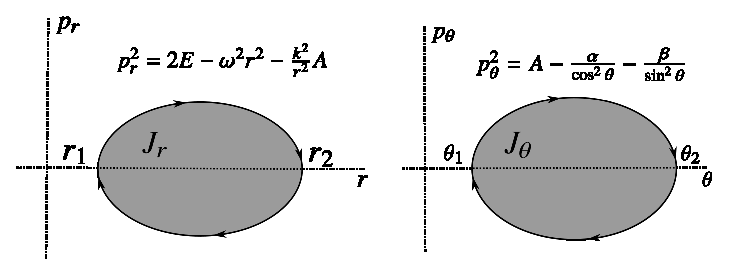
\includegraphics[width=\textwidth]{ciclos} 
  \end{frame}

  \begin{frame}{Superintegrabilidad del sistema de TTW}
    Toros de Liouville con $H=E$ y $X_k=k^2 A$:
    \begin{equation*}
      \begin{cases}
	p_r^2 + \dfrac{k^2}{r^2}A + \omega^2 r^2 = 2E, \\[5 pt]
	p_\theta^2 + \dfrac{\alpha}{\cos^2 \theta}+ \dfrac{\beta}{\sen^2 \theta} = A.
      \end{cases}
    \end{equation*}

    \begin{align*}
      J_r&=\frac{1}{2\pi} \oint \sqrt{2E-\omega^2 r^2 - \frac{k^2}{r^2}A} dr = \frac{E}{2\omega}- \frac{k\sqrt{A}}{2}, \\
      J_\theta&= \frac{1}{2\pi} \oint \sqrt{A-\frac{\alpha}{\cos^2 \theta}-\frac{\beta}{\sen^2 \theta}}d\theta = \frac{\sqrt{A}}{2}- \frac{\sqrt{\alpha}+\sqrt{\beta}}{2}\sim \frac{\sqrt{A}}{2}.
    \end{align*}
    
  \end{frame}

  \begin{frame}{Superintegrabilidad del sistema de TTW}
    \begin{equation*}
      H(J_r,J_\theta,w_r,w_\theta)=2\omega(J_r+kJ_\theta).
    \end{equation*}
    \pause
    \begin{equation*}
      \begin{cases}
	\nu_r=\dot{w}_r=\dfrac{\partial H}{\partial J_r}= 2\omega, \\[7 pt]
	\nu_\theta=\dot{w}_\theta=\dfrac{\partial H}{\partial J_\theta}= 2k\omega.
      \end{cases}
    \end{equation*}
    \pause
    \begin{itemize}
      \item $k$ irracional $\implies$ $\nu_r$, $\nu_\theta$ inconmesurables $\implies$ Trayectorias densas $\implies$ No superintegrable
    \pause
      \item $k=m/n$ $\implies$ $m\dot{w_r}-n\dot{w_\theta}=0$ $\implies$ $mw_r-nw_\theta$ es una cantidad conservada $\implies$
      $e^{i(mw_r - nw_{\theta})}=(e^{iw_r})^m(e^{-iw_\theta})^n$
    es una cantidad conservada univaluada en el toro de Liouville.
    \end{itemize}

  \end{frame}

  \begin{frame}{TTW en coordenadas complejas}
    \begin{equation*}
      z= x+ iy, \ \ \bar{z} = x- iy.
    \end{equation*}
    \pause
    \begin{equation*}
      \cos k\phi = \frac{z^k + \bar{z}^k}{2 |z|^k}, \ \ \sen k\phi = \frac{z^k - \bar{z}^k}{2i |z|^k}.
    \end{equation*}
    \pause
    \begin{equation*}
      V_k(z,\bar{z})=2k^2 z^{k-1}\bar{z}^{k-1}\left[ \frac{\alpha}{(z^k+\bar{z}^k)^2}-\frac{\beta}{(z^k-\bar{z}^k)^2} \right].
    \end{equation*}
    \pause
    \begin{equation*}
      T(z,\bar{z},\dot{z},\dot{\bar{z}})=\tfrac{1}{2}\dot{z}\dot{\bar{z}}.
    \end{equation*}
    \pause
    \begin{equation*}
      \begin{cases}
	p_z=\dfrac{\partial T}{\partial \dot{z}}= \frac{1}{2}(p_x-ip_y),\\[5 pt]
      p_{\bar{z}}=\dfrac{\partial T}{\partial \dot{\bar{z}}}= \frac{1}{2}(p_x+ip_y).
    \end{cases}
    \end{equation*}
    \pause
    \begin{equation*}
      H_k(z,\bar{z},p_z,p_{\bar{z}})=\tfrac{1}{2}(p_zp_{\bar{z}}+\omega^2 z \bar{z})+ V_k(z,\bar{z}).
    \end{equation*}
  \end{frame}

  \begin{frame}{TTW en unas nuevas coordenadas}
    \begin{equation*}
	u=\frac{1}{2}(z^k+\bar{z}^k)=r^k\cos k\phi, \ \
	v=\frac{1}{2}(z^k-\bar{z}^k)=r^k\sin k\phi
    \end{equation*}
    \pause
    \begin{equation*}
      \dot{u}=\frac{k}{2}(z^{k-1}\dot{z}+\bar{z}^{k-1}\dot{\bar{z}}), \ \
      \dot{v}=\frac{k}{2i}(z^{k-1}\dot{z}-\bar{z}^{k-1}\dot{\bar{z}}). \ \
    \end{equation*}
    \pause
    \begin{equation*}
      T(u,v,\dot{u},\dot{v})=\frac{\dot{u}^2+\dot{v}^2}{2k^2(u^2+v^2)^{(k-1)/k}}
    \end{equation*}
    \pause
    \begin{align*}
      p_u&=\frac{\partial T}{\partial \dot{u}}=\frac{\dot{u}}{k^2(u^2+v^2)^{(k-1)/k}}\\
      p_v&=\frac{\partial T}{\partial \dot{v}}=\frac{\dot{v}}{k^2(u^2+v^2)^{(k-1)/k}}
    \end{align*}
    \pause
    \begin{equation*}
      V_k(u,v)=k^2(u^2+v^2)^{(k-1)/k}\left[ \frac{\alpha}{2u^2}+\frac{\beta}{2v^2} \right].
    \end{equation*}
  \end{frame}
  \begin{frame}{TTW en unas nuevas coordenadas}
    \begin{equation*}
      H_k=k^2(u^2+v^2)^{(k-1)/k}\left[ \tfrac{1}{2}(p_u^2+p_v^2)+\frac{\omega^2}{2k^2}(u^2+v^2)^{2/k-1}+\frac{\alpha}{2u^2}+\frac{\beta}{2v^2} \right].
    \end{equation*}
    \pause
   Aparte del factor global $k^2(u^2+v^2)^{(k-1)/k}$, obtenemos un oscilador no lineal con términos centrífugos, que nos plantea varias preguntas
    \pause
   \begin{itemize}
     \item ¿Cuál es su origen?
    \pause
     \item ¿Cuál es su sentido físico?
    \pause
     \item ¿Se puede obtener de la reducción de un sistema en dimensión superior?
    \pause
     \item ¿Se puede interpretar como un factor conforme de un espacio curvo?
   \end{itemize}
    
  \end{frame}
  
  \begin{frame}{Espacios de curvatura constante}
    Modelizamos los espacios de curvatura constante $\kappa$ con la familia de superficies $\Sigma_\kappa \subset \mathbb{R}^3$ de ecuación
    \begin{equation*}
      x_0^2+\kappa(x_1^2+x_2^2)=1,
    \end{equation*}
    dotadas de la estructura riemanniana
    \begin{equation*}
      ds^2=\frac{1}{\kappa}(\mathrm{d}x_0^2+\mathrm{d}x_1^2+\mathrm{d}x_2^2)=\frac{\kappa(x_1\mathrm{d}x_1+x_2\mathrm{d}x_2 )^2}{1-\kappa (x_1^2+x_2^2)}+\mathrm{d}x_1^2+\mathrm{d}x_2^2.
    \end{equation*}
    \pause
    \begin{itemize}
      \item Si $\kappa>0$ tenemos modelos de la geometría esférica $\mathbb{S}^2$.
    \pause
      \item Si $\kappa=0$ tenemos dos planos, de los cuales escogemos uno, que nos da un modelo de la geometría euclidiana $\mathbb{E}^2$.
    \pause
      \item Si $\kappa<0$ obtenemos un hiperboloide de dos hojas, de las cuales escogemos una, que nos da un modelo del plano hiperbólico $\mathbb{H}^2$.
    \end{itemize}
  \end{frame}

  \begin{frame}{Espacios de curvatura constante}
    Modelizamos los espacios de curvatura constante $\kappa$ con la familia de superficies $\Sigma_\kappa \subset \mathbb{R}^3$ de ecuación
    \begin{equation*}
      x_0^2+\kappa(x_1^2+x_2^2)=1,
    \end{equation*}
    dotadas de la estructura riemanniana
    \begin{equation*}
      ds^2=\frac{1}{\kappa}(\mathrm{d}x_0^2+\mathrm{d}x_1^2+\mathrm{d}x_2^2)=\frac{\kappa(x_1\mathrm{d}x_1+x_2\mathrm{d}x_2 )^2}{1-\kappa (x_1^2+x_2^2)}+\mathrm{d}x_1^2+\mathrm{d}x_2^2.
    \end{equation*}
    La energía cinética tiene entonces la forma
    \begin{equation*}
      T_{\kappa}(x_1,x_2,\dot{x}_1,\dot{x}_2)=\frac{\kappa(x_1\dot{x}_1+x_2\dot{x}_2 )^2}{2[1-\kappa (x_1^2+x_2^2)]}+\frac{1}{2}(\dot{x}_1^2+\dot{x}_2^2).
    \end{equation*}
  \end{frame}

  \begin{frame}{Coordenadas polares geodésicas}
    Definimos las \emph{coordenadas polares geodésicas} $(\chi,\phi)$, dadas por la relación
    \begin{equation*}
      \begin{cases}
	x_1=s_{\kappa}(\chi)\cos\phi,\\
	x_2=s_{\kappa}(\chi)\sen\phi,
      \end{cases}
    \end{equation*}
    donde $s_{\kappa}$ es una de las \emph{funciones trigonométricas generalizadas}
 \begin{equation*}
  c_{\kappa}(\chi)=
  \begin{cases}
    \cos \sqrt{\kappa} \chi & \kappa >0, \\
    1 & \kappa =0, \\
    \cosh \sqrt{-\kappa} \chi & \kappa <0, 
  \end{cases}
  \ \ \ 
  s_{\kappa}(\chi)=
  \begin{cases}
    \frac{1}{\sqrt{\kappa}}\sen \sqrt{\kappa} \chi & \kappa >0, \\
    \chi & \kappa =0, \\
    \frac{1}{\sqrt{-\kappa}}\senh \sqrt{-\kappa} \chi & \kappa <0. 
  \end{cases}
\end{equation*}
 \end{frame}

 \begin{frame}{Coordenadas polares geodésicas}
   \centering
   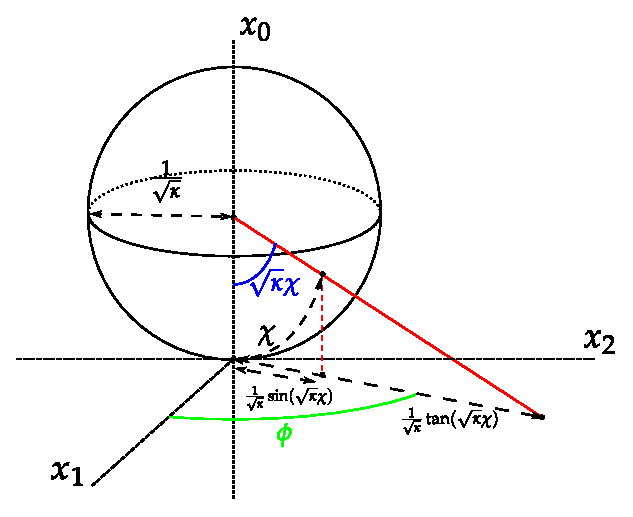
\includegraphics{esfera}
 \end{frame}

 \begin{frame}{Coordenadas polares geodésicas}
  En estas coordenadas la energía cinética toma la forma
  \begin{equation*}
    T_{\kappa}(\chi,\phi,\dot{\chi},\dot{\phi})=\tfrac{1}{2}(\dot{\chi}^2+s_{\kappa}^2(\chi)\dot{\phi}^2).
  \end{equation*}
  \pause
 Los momentos conjugados de las coordenadas polares geodésicas vendrán dados por
 \begin{align*}
   p_{\chi}=\frac{\partial T_{\kappa}}{\partial \dot{\chi}}= \dot{\chi} \\
   p_{\phi}=\frac{\partial T_{\kappa}}{\partial \dot{\phi}}= s_\kappa^2(\chi)\dot{\phi}. 
 \end{align*}
  \pause
 Por tanto, el hamiltoniano libre es
 \begin{equation*}
   H_{\kappa}(\chi,\phi,p_\chi,p_\phi)=\frac{1}{2}\left( p_{\chi}^2 + \frac{p_\phi ^2}{s_\kappa^2(\chi)} \right).
 \end{equation*}
  
 \end{frame}

 \begin{frame}{TTW en espacios de curvatura constante}
   Podemos generalizar el hamiltoniano de TTW a los espacios de curvatura constante en la forma
   \begin{equation*}
     H_{k,\kappa}(\chi,\phi,p_\chi,p_\phi)=\frac{1}{2}\left( p_\chi^2+ \frac{p_\phi^2}{s^2_{\kappa}(\chi)}+\omega^2 t^2_{\kappa}(\chi) \right)+V_{k,\kappa}(\chi,\phi),
   \end{equation*}
   donde $t_k=s_k/c_k$ y
   \begin{equation*}
     V_{k,\kappa}(\chi,\phi)=\frac{k^2 \alpha}{2s_{\kappa}^2(\chi)\cos^2k\phi}+\frac{k^2 \beta}{2s_{\kappa}^2(\chi)\sen^2k\phi}.
   \end{equation*}

  \pause
   Nótese que en el límite euclidiano (cuando $\kappa\rightarrow 0$), se recupera el hamiltoniano de TTW en el plano.
 \end{frame}

 \begin{frame}{Referencias}
   \nocite{*}
   \bibliographystyle{aip2}
   \bibliography{biblio}
 \end{frame}

 \begin{frame}
   \centering
   \Huge ¿PREGUNTAS?
 \end{frame}
\end{document}
